%%%
% Author: Yihong Liu (https://liu-yihong.github.io/)
% Repository:
% License: GNU GPL v3.0
% This repository contains an unofficial LaTex beamer
% template for the University of Texas at Dallas.
% Copyright (c) 2022 Yihong Liu
%%%
\documentclass[
	xcolor={svgnames},
	hyperref={pagebackref,bookmarks},
	% aspectratio=169,
	aspectratio=43,
]{beamer}

\mode<presentation>
%%%
% Author: Yihong Liu (https://liu-yihong.github.io/)
% Repository:
% License: GNU GPL v3.0
% This repository contains an unofficial LaTex beamer template for the University of Texas at Dallas.
% Copyright (c) 2022 Yihong Liu
%%%
\usepackage[utf8]{inputenc}
\usepackage{xcolor}
\usepackage{tikz}
% \usepackage{fontawesome5}
\usepackage{fontawesome}
%%%
% Author: Yihong Liu (https://liu-yihong.github.io/)
% Repository:
% License: GNU GPL v3.0
% This repository contains an unofficial LaTex beamer template for the University of Texas at Dallas.
% Copyright (c) 2022 Yihong Liu
%%%
\usetheme{AnnArbor} % Dresden Berlin Madrid Singapore Frankfurt Montpellier
\usecolortheme{crane}
% https://www.cpt.univ-mrs.fr/~masson/latex/Beamer-appearance-cheat-sheet.pdf
\definecolor{utdorange}{RGB}{232,117,0}
\definecolor{utdgreen}{RGB}{18,71,52}
\definecolor{utdcyan}{RGB}{95,244,183}
\definecolor{utdcyangray}{RGB}{138,141,143}

\setbeamercolor*{structure}{bg=utdorange!40,fg=utdorange}

\setbeamercolor*{palette primary}{use=structure,fg=white,bg=structure.fg}
\setbeamercolor*{palette secondary}{use=structure,fg=white,bg=structure.fg!75}
\setbeamercolor*{palette tertiary}{use=structure,fg=white,bg=utdgreen}
\setbeamercolor*{palette quaternary}{fg=white,bg=structure.fg}

\setbeamercolor*{palette sidebar primary}{use=structure,fg=white,bg=structure.fg}
\setbeamercolor*{palette sidebar secondary}{use=structure,fg=white,bg=structure.fg!75}
\setbeamercolor*{palette sidebar tertiary}{use=structure,fg=white,bg=utdgreen}
\setbeamercolor*{palette sidebar quaternary}{fg=white,bg=structure.fg}

\setbeamercolor*{section in toc}{fg=black,bg=white}
% \setbeamercolor{alerted text}{use=structure,fg=utdcyan}
\setbeamercolor{block title alerted}{use=structure,bg=utdcyan}

\setbeamercolor{titlelike}{parent=palette primary,fg=white,bg=utdorange}
\setbeamercolor{frametitle}{bg=utdorange!85,fg=white}
% \setbeamercolor*{titlelike}{parent=palette primary}
%%%
% Author: Yihong Liu (https://liu-yihong.github.io/)
% Repository:
% License: GNU GPL v3.0
% This repository contains an unofficial LaTex beamer template for the University of Texas at Dallas.
% Copyright (c) 2022 Yihong Liu
%%%
% https://tex.stackexchange.com/questions/443659/how-to-remove-date-from-footnote-of-madrid-theme-of-beamer-and-use-that-space-fo
\makeatletter
\setbeamertemplate{footline}{%
  \leavevmode%
  \hbox{%
    \begin{beamercolorbox}[wd=.15\paperwidth,ht=2.25ex,dp=1ex,center]{author in head/foot}{CS5150}%
%      \usebeamerfont{author in head/foot}\insertshortauthor\expandafter\ifblank\expandafter{\beamer@shortinstitute}{}{~~\insertshortinstitute}
    \end{beamercolorbox}%
    \begin{beamercolorbox}[wd=.77\paperwidth,ht=2.25ex,dp=1ex,center]{title in head/foot}%
      \usebeamerfont{title in head/foot}\insertshorttitle
    \end{beamercolorbox}%
  }%
  \begin{beamercolorbox}[wd=.08\paperwidth,ht=2.25ex,dp=1ex,right]{date in head/foot}%
    \usebeamerfont{date in head/foot}%
    \usebeamertemplate{page number in head/foot}%
    \hspace*{2ex}
  \end{beamercolorbox}
  \vskip0pt%
}
\makeatother
%gets rid of bottom navigation symbols
\setbeamertemplate{navigation symbols}{}
%gets rid of bottom navigation bars
% \setbeamertemplate{footline}[frame number]{}
%gets rid of footer
% \setbeamertemplate{footline}{}
%%%
% Author: Yihong Liu (https://liu-yihong.github.io/)
% Repository:
% License: GNU GPL v3.0
% This repository contains an unofficial LaTex beamer template for the University of Texas at Dallas.
% Copyright (c) 2022 Yihong Liu
%%%
\newcommand{\presentationtitle}{}
\newcommand{\presentationsubtitle}{}
\newcommand{\presenter}{}
\newcommand{\department}{}
\newcommand{\school}{}
\newcommand{\university}{}
\newcommand{\email}{}
\renewcommand{\presentationtitle}{Markov Chain Approximations to Evaluate CCN Caching Systems}
\renewcommand{\presenter}{Jatin Tarachandani, Taha Adeel Mohammed}
\renewcommand{\department}{Computer Science and Engineering}
\renewcommand{\school}{IITH}
\renewcommand{\university}{Indian Institute of Technology Hyderabad}
\renewcommand{\email}{\href{mailto:cs20btech11052@iith.ac.in}}
%%%
% Author: Yihong Liu (https://liu-yihong.github.io/)
% Repository:
% License: GNU GPL v3.0
% This repository contains an unofficial LaTex beamer template for the University of Texas at Dallas.
% Copyright (c) 2022 Yihong Liu
%%%
\hypersetup{
    pdfauthor={\presenter},%
    pdftitle={\presentationtitle - \presentationsubtitle},%
    pdfsubject={\department},%
    pdfkeywords={\department, \school, \university},%
    pdfproducer={LaTeX},%
    pdfcreator={pdfLaTeX},
    % bookmarks,
    bookmarksnumbered = true,
    bookmarksopen     = true,
    % pdfpagelabels     = true,
    pdfstartview={XYZ null null 1.2}
}

%% End of Template

\usepackage{blkarray}
\usepackage{amsmath}
\usepackage{amsfonts}
\usepackage{amssymb}
\usepackage{mathtools}

\title[]{Markov Chain Approximations to Evaluate CCN Caching Systems}

\title{\presentationtitle}
\author{\presenter}
\institute[IITH]{
	\university\\
}
\date{\today}

\makeatletter
\makeatother

\begin{document}

\AtBeginSection[]{
    \begin{frame}
        \vfill
        \centering
        \begin{beamercolorbox}[sep=8pt,center,shadow=true,rounded=true]{title}
        \usebeamerfont{title}\insertsectionhead\par%
        \end{beamercolorbox}
        \vfill
    \end{frame}
}

\newcommand{\brak}[1]{\ensuremath{\left( #1 \right)}}
\newcommand{\sbrak}[1]{\ensuremath{\left[ #1 \right]}}
\newcommand{\Exp}[1]{\ensuremath{\mathbb{E} \left[ #1 \right]}}
\newcommand{\Var}[1]{\ensuremath{\text{Var} \left[ #1 \right]}}
\setbeamercolor{alerted text}{fg=orange}

\begin{frame}
	\titlepage
\end{frame}


\begin{frame}{Reference}
    \begin{block}{\textbf{Title}}
        A versatile Markov chain model for the performance analysis of CCN caching systems
    \end{block}
    \begin{block}{\textbf{Authors}}
        \begin{itemize}
            \item Hamza Ben-Ammar - University of Rennes, IRISA, France
            % Yassine Hadjadj-Aoul, Gerardo Rubino and Soraya Ait-Chellouche
            \item Yassine Hadjadj-Aoul - University of Rennes
            \item Gerardo Rubino - University of Rennes
            \item Soraya Ait-Chellouche - University of Rennes
        \end{itemize}
    \end{block}
    \begin{block}{\textbf{Year of Publication}}
        \begin{itemize}
            \item 2018
        \end{itemize}
    \end{block}
\end{frame}

\begin{frame}{Contents}
	\tableofcontents
\end{frame}


\section{Introduction}
\subsection*{CCN}
\begin{frame}{Introduction}
	\begin{block}{\textbf{CCN?}}
		\begin{itemize}
		    \item \textbf{C}ontent \textbf{C}entric \textbf{N}etworking
            \item Here, network of nodes (graph representable)
            \item Nodes have their own distinct caches
            \item Some nodes have attached content repositories (final destination)
            \item Requests transmitted across network via \textit{interest packets}, and corresponding \textit{data packets} cached (or not) at nodes along which response is sent
            \item Above point depends on caching strategy
		\end{itemize}
	\end{block}
\end{frame}

\subsection*{Motivation and Terminology}
\begin{frame}{Introduction}
    \begin{block}{\textbf{Why CCN?}}
        \begin{itemize}
            \item Allows to focus more on content itself rather than location
            \item Intermediate caching reduces round-trip time and server load
            \item Achieves significant improvements \footnotemark
        \end{itemize}
    
    \end{block}
    \begin{block}{\textbf{Other Related Terminology}}
        \begin{itemize}
            \item LCE: \textbf{L}eave \textbf{C}opy \textbf{E}verywhere - caching strategy that basically means whenever a data comes as a response through a node, cache a copy
            \item LRU - \textbf{L}east \textbf{R}ecently \textbf{U}sed - individual nodes' cache replacement algorithm considered in this work 
        \end{itemize}
    \end{block}
    \footnotetext{G. Rossini and D. Rossi, “A dive into the caching performance of content centric networking,” in Proc. of IEEE CAMAD, Sep. 2012, pp. 105–109.}
\end{frame}

\subsection*{High Level Overview}
\begin{frame}{Introduction}
\begin{block}{\textbf{Markov Chain Analysis of this System} (High-level)}
    \begin{itemize}
        \item We consider a r-ranked set of content $\{c_r\}, r \in \{1, 2, ... R\}$. Probability of requesting any one $\rightarrow$ $p_r$. 
        \item Goal - Approximate the cache hit ratio for a content $c_r$ and validate against simulation numbers
        \item DTMCs used to model a \textit{single cache node}
        \begin{itemize}
            \item One DTMC constructed per content item
            \item Transition probabilities dependent on $p_r$
        \end{itemize}
        \item Further generalization to a system of cache nodes forming the network
    \end{itemize}
\end{block}
\end{frame}

\section{System Description}
\begin{frame}{System Description}
    \begin{block}{\textbf{Notations}}
        \begin{itemize}
            \item $G = (V, E)$: Graph representing the network of caches
            \item $V = \{v_1, \ldots,  v_M\}$: Set of nodes, each with a cache
            \item $E \subseteq V \times V$: Set of links between nodes
            \item $C = \{c_1, \ldots, c_R\}$: Set of content items
            \item $p_r$: Probability of requesting content $c_r$
            \item $N$: Size of the cache for each node, where $N << R$
            \item $\beta(r)$: Probability that $c_r$ is cached at a node upon a cache miss
        \end{itemize}
    \end{block}
\end{frame}

\begin{frame}{System Description}
    \begin{itemize}
        \item All content items $c_r$ have an identical size and are stored permanently at some nodes (servers) in the network.
        \item The clients generate independent and identically distributed sequence of requests from the catalog of content items. (\textbf{IRM} - \textbf{I}ndependent \textbf{R}eference \textbf{M}odel) \footnotemark
        \item \textbf{Shortest Path Routing:} Each node has a \textbf{F}orwarding \textbf{I}nformation \textbf{B}ase (FIB) table that contains the next hop for each content item.
        % Pending Interest Table (PIT) is used to store the pending requests.
        \item \textbf{LRU Replacement:} The cache replacement policy is Least Recently Used (LRU).
    \end{itemize}
    \footnotetext{A. Dan and D. Towsley, “An approximate analysis of the LRU and FIFO buffer replacement schemes,” \textit{SIGMETRICS}, vol. 18, pp. 143-152, Apr. 1990}
\end{frame}

\begin{frame}
    \begin{itemize}
        \item \textbf{Zipf's Law:} The content catalog $C$ has an inherent popularity ranking following the Zipf distribution\footnotemark.
    \end{itemize}
    \begin{columns}
        \column{0.3\linewidth}
        \begin{align*}
            &p_r = \frac{r^{-\alpha}}{\sum_{r=1}^{R} r^{-\alpha}}, \text{ where } \\
            c_r \rightarrow& \text{ content with popularity rank } r \\
            p_r \rightarrow& \text{ probability of requesting } c_r \\ 
            \alpha \rightarrow& \text{ skewness of the Zipf distribution}
        \end{align*}
        \column{0.4\linewidth}
        \begin{figure} \vspace*{-7mm}
            \centering
            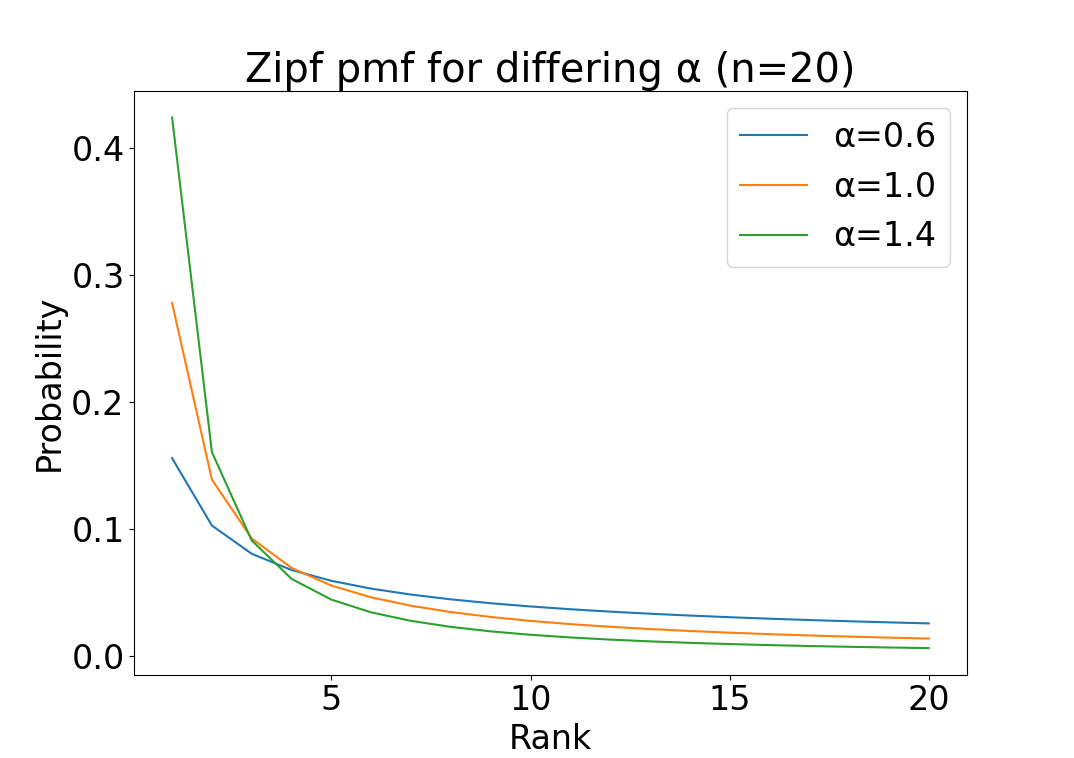
\includegraphics[scale=0.2]{zipf.png}
        \end{figure}
    \end{columns}
    \footnotetext{F. Guillemin, T. Houdoin, and S. Moteau, “Volatility of youtube content in orange networks and consequences,” \textit{2013 IEEE International Conference on Communications}}
\end{frame}

\section{Single Node Cache Analysis}
\subsection*{Introduction}
\begin{frame}{Single Node Cache Analysis}
    % When a cache hit/caching decision happens, the item is moved to the top of the cache.
    Given an LRU Cache with size $N$, when a content $c_r$ is requested and recieved at a node, for any $c_{r'}$ (with $r' \neq r$) at position $i$ in the cache, the following cases arise:
    \begin{itemize}
        \item $c_{r'}$ is moved down by one position if $c_r$ is not in the cache and $c_r$ is being cached currently (with prob. $\beta(r)$), or if $c_r$ is at $j$ with $j > i$.
        \item $c_{r'}$ will remain at the same position if $c_r$ is at $j$ with $j < i$ or if it has been decided to not cache $c_r$ (with prob. $1 - \beta(r)$).
        \item $c_{r'}$ will be evicted if it occupies the $N^{th}$ position and $c_r$ is not in the cache and $c_r$ is being cached currently (with prob. $\beta(r)$).
    \end{itemize}
\end{frame}

\subsection*{Markov Chain Model}
\begin{frame}{MACS}
    \begin{itemize}
        \item \textit{Configuration:} $\vec{x} = (x_1, x_2, \ldots, x_N)$, where $x_i$ is the content item at position $i$ in the cache.
        \item $|Configurations| = R!/(R-N)!$ \quad Huge!!
    \end{itemize}
    \begin{block}{\textbf{M}arkov chain-based \textbf{A}pproximation of CCN \textbf{C}aching \textbf{S}ystem \textbf{(MACS)}}
        \begin{itemize}
            \item Consider a Markov chain $X(r)$ with N+1 states.
            \item The chain represents the evolution with time of the position occupied by $c_r$ in the cache.
            \item State 1 means that $c_r$ is at the top of the cache, $\ldots$ , state $N$ means that $c_r$ is at the bottom of the cache.
            \item State $N+1$ means that $c_r$ is not in the cache.
            \item The chains $X(1), X(2), \ldots , X(R)$ are independent of each other.
        \end{itemize}
    \end{block}
\end{frame}

\subsection*{Transition Probabilities}
\begin{frame}{Transition Probabilities}
    \begin{columns}
        \column{0.03\linewidth}
        \column{0.5\linewidth}
        \textbf{\underline{Definition}: \boldmath$\gamma_s(r)$} \\ \vspace*{1mm}
            $\gamma_s(r) \rightarrow$ probability that content $c_r$ stays at the same state $s$ in $X(r)$, when $\beta(r) = 1$
            \begin{equation}
                \begin{dcases*}
                    \gamma_1(r) = p_r, \\
                    \gamma_s(r) = \sum_{i = 1, i \neq r}^{R} \!\!\!p_i\!\sum_{j = 1}^{s - 1} \pi_j(i), \, s \in \lbrack2, N\rbrack, \\
                    \gamma_{N+1}(r) = 1 - p_r.
                \end{dcases*}
            \end{equation}
        \column{0.5\linewidth}
        \begin{figure}
            \centering
            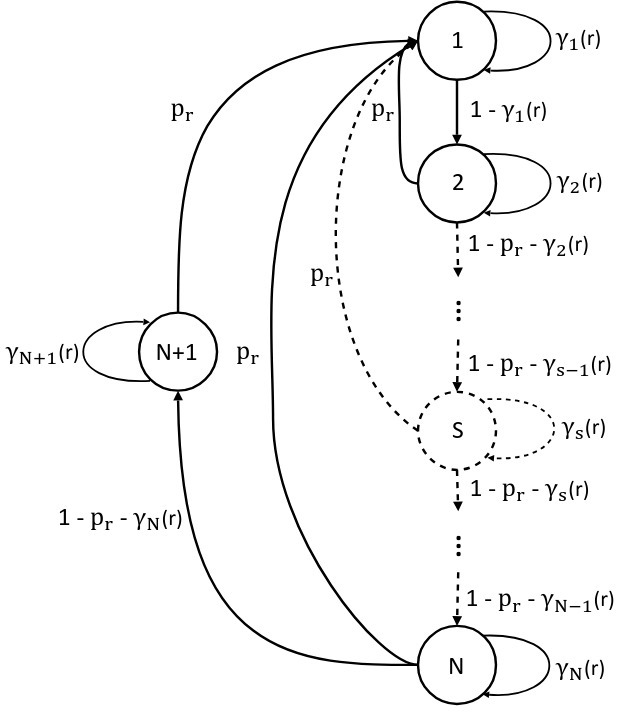
\includegraphics[scale=0.24]{macs0.jpeg}
        \end{figure}
    \end{columns}
\end{frame}

\begin{frame}{Transition Probabilities}
    \begin{columns}
        \column{0.03\linewidth}
        \column{0.5\linewidth}
        \textbf{\underline{Definition}: \boldmath$\gamma_s'(r)$} \\ \vspace*{1mm}
            $\gamma_s'(r) \rightarrow$ probability that content $c_r$ stays at the same state $s$ in $X(r)$
            \begin{equation}
                \begin{dcases*}
                    \gamma_s'(r)\! =\! \gamma_s(r)\! + \mkern-18mu \sum_{i = 1, i \neq r}^{R}\mkern-10mu p_i \pi_{N+1}(i)(1\!\! -\!\! \beta(i)), \\
                    \gamma_{N+1}'(r) = 1 - p_r\beta(r).
                \end{dcases*}
            \end{equation}
            where $\pi_{N+1}(i)$ is the probability that $c_i$ is not in the cache.
            % This is an approximation, since pi_N+1 is being used to compute pi_N+1 
        \column{0.5\linewidth}
        \begin{figure}
            \centering
            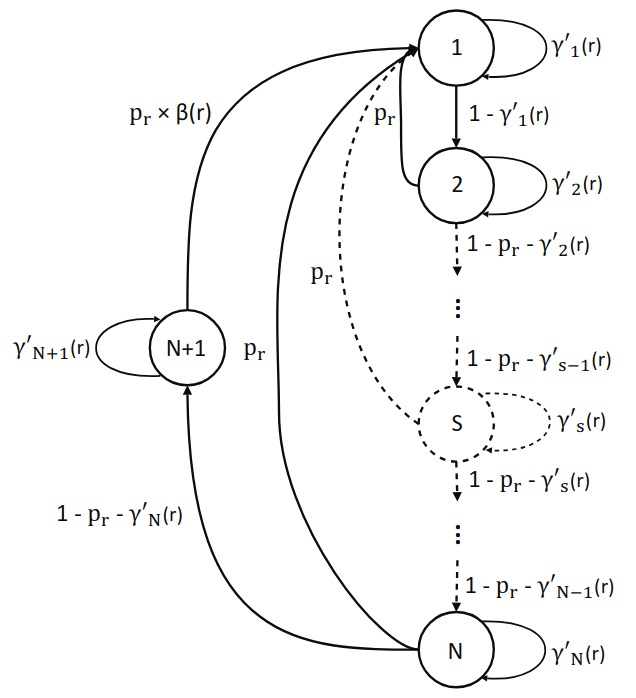
\includegraphics[scale=0.25]{macs.jpeg}
        \end{figure}
    \end{columns}
\end{frame}

\begin{frame}{Transition Probabilities}
    \begin{columns}
        \column{0.03\linewidth}
        \column{0.5\linewidth}
        \textbf{\underline{Definition}: \boldmath$T_{i, j}$} \\ \vspace*{1mm}
            $T_{i, j} \rightarrow$ Transition probability from state $i$ to state $j$ in $X(r)$
            \begin{equation}
                \begin{dcases*}
                    \quad\,\,\, T_{i, i} = \gamma_i'(r), \qquad\,\, i \in \lbrack 1, N+1 \rbrack, \\
                    \quad\,\, T_{i, 1} = p_r, \quad\qquad\qquad\,\, i \in \lbrack 2, N \rbrack, \\
                    T_{N+1, 1} = p_r \beta(r), \\
                    \quad\, T_{1, 2} = 1 - \gamma_1'(r), \\
                    \,\,\,T_{i, i+1} = 1 - p_r - \gamma_i'(r), \,\,\, i \in \lbrack 2, N \rbrack, \\
                    \quad\ \, T_{i, j} = 0, \qquad\quad\,\,\ j \notin \lbrace 1, i, i+1 \rbrace.
                \end{dcases*}
            \end{equation}
        \column{0.5\linewidth}
        \begin{figure}
            \centering
            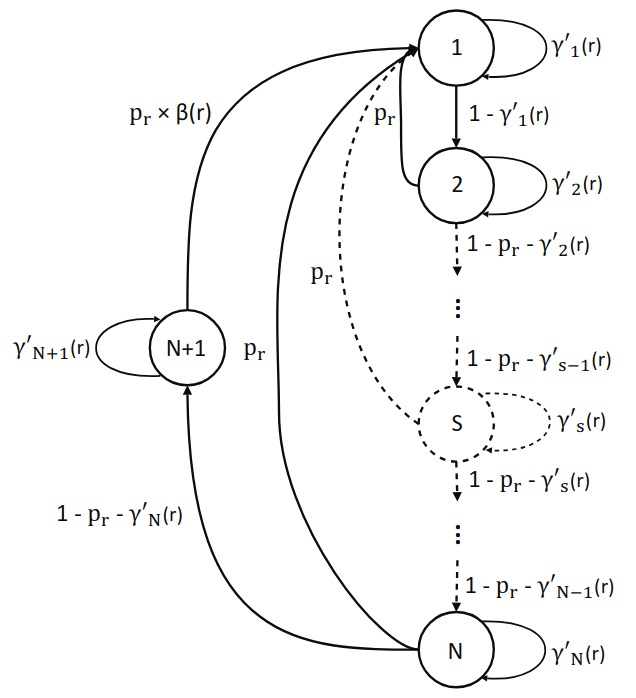
\includegraphics[scale=0.25]{macs.jpeg}
        \end{figure}
    \end{columns}
\end{frame}

\subsection*{Stationary Distribution}
\begin{frame}{Stationary Distribution}
    \begin{block}{\textbf{Stationary Distribution Existence}}
        \begin{itemize}
            \item From the markov chain, we can see that the states form a SCC and hence the chain is irreducible. 
            \item Also, due to self loops, the chain is aperiodic. ($0 < \gamma_s'(r) < 1$) 
            \item Hence, the chain is ergodic and has a unique stationary distribution $\pi(r) = (\pi_1(r), \pi_2(r), \ldots, \pi_{N+1}(r))$.
            \item The cache miss probability would be given by $\pi_{N+1}(r)$ and the cache hit rate by $(1 - \pi_{N+1}(r))$.
        \end{itemize}
    \end{block}
\end{frame}

\begin{frame}{Stationary Distribution}
    \begin{block}{\textbf{Stationary Equations}}
        Using the Chapman-Kolmogorov equations ($\pi = \pi P$ and $\sum\pi_i = 1$) and the transition probabilities derived earlier, we obtain:
        \begin{equation}
            \begin{dcases*}
                \pi_1(r) = \pi_1(r)\gamma_1'(r) + \sum_{i=2}^{N} \pi_i(r)p_r + \pi_{N+1}(r)p_r\beta(r) \\
                \pi_2(r) = \frac{\pi_1(r)(1 - \gamma_1'(r))}{1 - \gamma_2'(r)} \\
                \pi_i(r) = \frac{\pi_{i-1}(r)(1 - p_r - \gamma_{i-1}'(r))}{1 - \gamma_i'(r)}, \, i \in \lbrack 3, N+1 \rbrack \\
                \pi_1(r) + \pi_2(r) + \cdots + \pi_{N+1}(r) = 1
            \end{dcases*}
        \end{equation}
        % We see that each $\pi_i(r)$ is a function of $pi_{i-1}$ (and hence $\pi_1(r)$), and hence we can solve for $\pi_1(r)$ and then get the rest of the values.
    \end{block}
\end{frame}

\begin{frame}{Stationary Distribution for LCE}
    For the LCE caching strategy, $\beta(r) = 1$ for all $r$. \vspace{-2mm}
    \begin{align}
        \implies \pi_1(r) = p_r
    \end{align}
    Hence, the system of equations derived earlier can be solved to get
    \begin{equation}
        \begin{dcases*}
            \pi_1(r) = p_r \\
            \pi_2(r) = \frac{p_r(1-p_r)}{1 - \gamma_2(r)} \\
            \pi_i(r) = \frac{p_r(1-p_r)\prod_{j=2}^{i-1}(1 - p_r - \gamma_j(r))}{\prod_{j=2}^{i}(1 - \gamma_j(r))}, \, i \in \lbrack 3, N+1 \rbrack
        \end{dcases*}
    \end{equation}
    % Complexity O(NR) for complete distribution
\end{frame}

\begin{frame}{Stationary Distribution Computation for Generic Case}
    \begin{itemize}
        \item In the general case of $0 \leq \beta(r) \leq 1$, $\pi_1(r)$ cannot be computed directly since it depends on all other $\pi_i(r)$.
        \item And each $\pi_{i \ge 2}(r)$ is a function of $\pi_{i-1}(r)$ (and hence $\pi_1(r)$).
        \item Hence to compute $\pi_1(r)$, the equations can be rearranged to get: \vspace*{-2.5mm}
        \begin{equation}
            \pi_1(r) = \frac{p_r(1 + (\beta(r) - 1)\pi_{N+1}(r))}{1 - (\gamma_1'(r) - \gamma_1(r))}
        \end{equation} 
        \item Now $\pi_1(r)$ depends only on $\pi_{N+1}(r)$.
        \item \textbf{Fixed Point Iteration:} Successive approximations of $\pi_{N+1}(r)$ can be used to get $\pi_1(r)$ and then the rest of the values.
        % Convergence is fast, i.e < 10 iterations
        % Computational complexity discuss
        % Approximations where all
        % Other assumptions?
    \end{itemize}
\end{frame}

\section{Multiple Nodes System}
\subsection*{Outgoing Miss Stream}
\begin{frame}{Multiple Nodes System}
    \begin{block}{\textbf{Extending to Multiple Cache Nodes}}
        \begin{itemize}
            \item So far, we derived for the states of a single cache node. 
            \item For multi-node network, we must consider request forwarding as another addition to $p_r$.
            \item Under SPR, we must consider requests from other nodes due to cache misses - miss stream or $MS_r$
        \end{itemize}
    \end{block}
    \begin{block}{\textbf{Definition}}
        The outgoing miss stream rate for a content $c_r$ from a node $u$ is:
        \begin{equation}
            MS_r(u) = req(r,u) \times \pi_{N+1}(r,u)
        \end{equation}
        where $req(r,u)$ is the proportion of requests for content $c_r$ received by $u$.
    \end{block}
\end{frame}

\subsection*{Incoming Miss Stream}
\begin{frame}{Incoming Miss Stream}
    \begin{block}{\textbf{Definition}}
        The incoming miss stream rate for content $c_r$ at node $v$ is:
        \begin{equation}
            \eta_r(v) = \sum_{u:NH(u)=v} \left( MS_r(u) \prod_{w \neq u:NH(w)=v} \left(1 - MS_r(w)\right)\right)
        \end{equation}
        \begin{itemize}
            \item $\{u:NH(u)=v\}$ is the set of nodes s.t. $u$'s \textbf{N}ext \textbf{H}op on the shortest path towards the repo location of $c_r$ is $v$.
            \item We take the $(1 - MS_r(w))$ terms due to request aggregation (duplicate requests collated, then forwarded)
        \end{itemize}
    \end{block}
\end{frame}

\subsection*{Adjusting $p_r$}
\begin{frame}{Adjusting $p_r$}
    \begin{itemize}
        \item As a result, node's content requests = client-origin requests + cache-miss-origin forwarded requests 
        \item Thus, value $p_r$ used in DTMC's $\pi_i(r)$ formula is no longer a valid probability of incoming requests
        \item It thus becomes (for each node $v$): 
        \begin{equation}
            p_r^\prime = \frac{p_r + \eta_r(v)}{\sum_{k=1}^R\left(p_k + \eta_k(v) \right)}
        \end{equation}
        and resubstitute $p_r^\prime$ in the original MC equations to get the adjusted $\pi$.
    \end{itemize}
\end{frame}

\section{Experimental Simulations}
\subsection*{Tools and parameters}
\begin{frame}{Simulator and Fixed Params}
    \begin{itemize}
        \item Simulations were conducted on \textit{ccnSim} \footnotemark, which is a discrete-event CCN simulator.
        \item Initially requests are sent until steady state (ccnSim checks this using batched Coeff. of Variation on $p_{\text{hit}}$), post which $10^6$ requests are sent. 
        \vspace{10pt}
        \begin{table}[]
            \centering
            \begin{tabular}{c|c}
            \hline
               Catalog size  & 20000 \\
               \hline
               Client model  & Poisson, 1req/s \\
               \hline
               $\beta(r)$  &  0.5 \\
               \hline
               Cache replacement  &  LRU \\
               \hline
            \end{tabular}
            \caption{Fixed Parameters}
            \label{tab:my_label}
        \end{table}
    \end{itemize}
    \footnotetext{Chiocchetti, Raffaele, Rossi, Dario and Rossini, Giuseppe, “ccnSim: an Highly Scalable CCN Simulator.” In IEEE International Conference on Communications (ICC), June 2013.}
\end{frame}

\subsection*{Variables / Topologies}
\begin{frame}{Variables / Topologies}
    Variables considered: 
    \begin{itemize}
        \item Zipf law skew parameter $\alpha$
        \begin{itemize}
            \item Values from 0.8 to 1.2
        \end{itemize}
        \item Cache size as a percentage of catalog size
        \begin{itemize}
            \item Values from 0.1\% to 1\%
        \end{itemize}
        \item Topology:
        \begin{itemize}
            \item 15-node binary tree
            \item 31-node binary tree
        \end{itemize}
        Here, clients are leaf nodes, repository is the root node
    \end{itemize}
\end{frame}

\subsection*{Results}
\begin{frame}{Result graphs}
    \begin{figure}
        \centering
        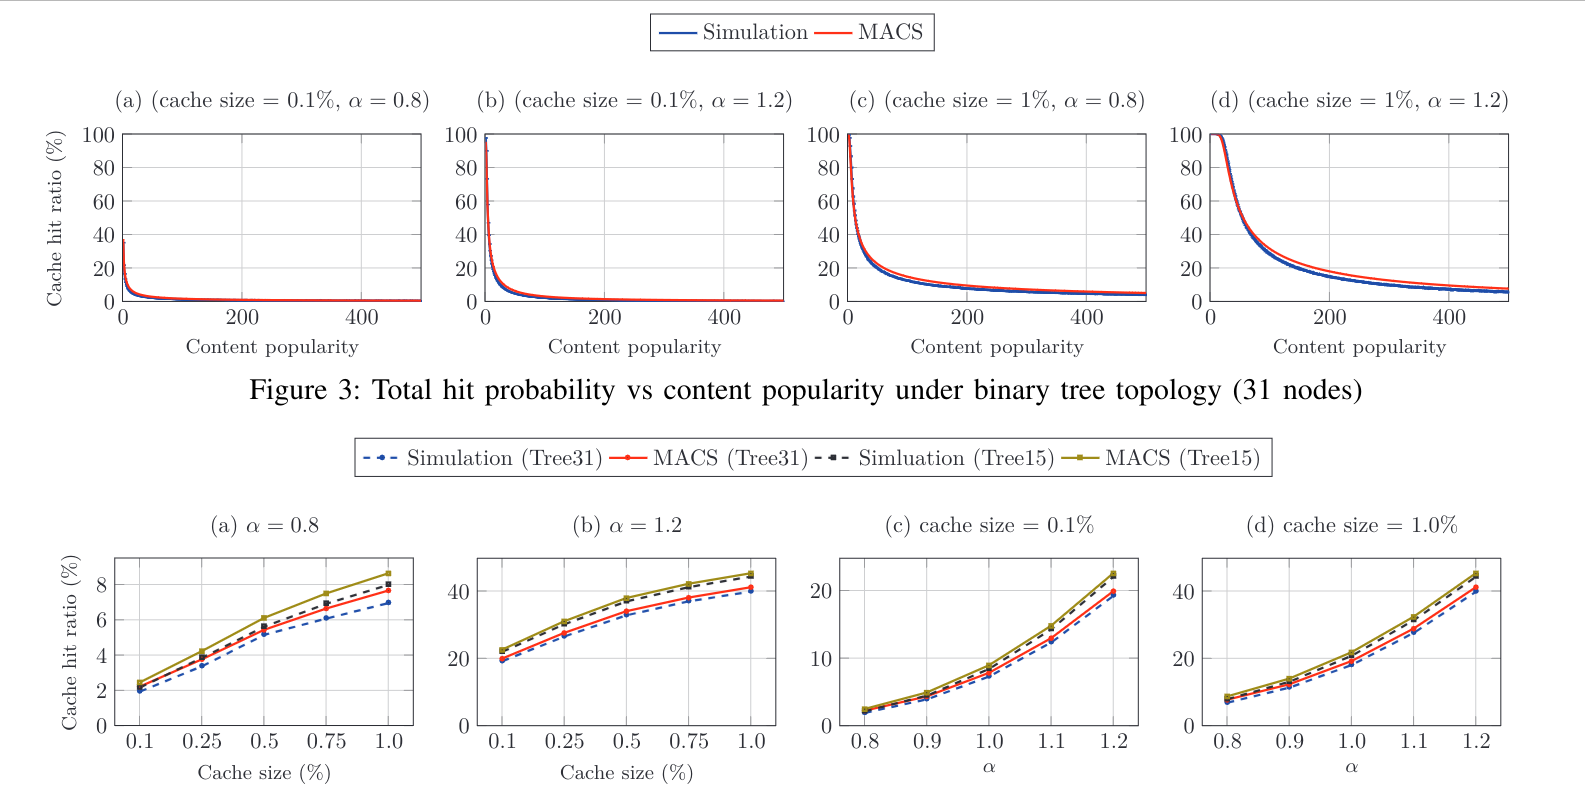
\includegraphics[scale=0.215]{benammarsimresults.png}
    \end{figure}
\end{frame}


\section{Our Work}

\subsection{Average Number of Hops for a Request}
\begin{frame}{Average Number of Hops for a Request}
    \begin{itemize}
        \item We build on the equilibrium distribution results $\pi(r)$ of MACS to get the average number of network hops before a request for content $c_r$ is satisfied.
        \item Let $\phi(u_0, c_r) = \lbrace u_0, u_1, \ldots , u_k \rbrace$ be the shortest route/path from $u_0$ to a server containing $c_r$.
        \item The expected number of hops for a request for $c_r$ from $u_0$ is:
        \begin{align}
            \Exp{H(u_0, c_r)} &= \sum_{i=0}^{k} i \times \prod_{j = 0}^{i-1} Pr(\text{Cache miss at }u_j) \times Pr(\text{Cache hit at }u_i) \nonumber \\
            &= \sum_{i=0}^{k} (i \times \prod_{j = 0}^{i-1} \pi_{N+1}(c_r, u_j) \times (1 - \pi_{N+1}(c_r, u_i)))
        \end{align}
    \end{itemize}
\end{frame}

\subsection{Advanced Topologies Simulations}
\begin{frame}{Evaluating on other graphs}
    \begin{itemize}
        \item Tree network topology considered is simplistic
        \item Average case topologies would be a better indicator of robustness of MACS 
        \item We do this by using random graphs for topologies
    \end{itemize}
\end{frame}

\begin{frame}{Barabási - Albert model\footnotemark}
    \begin{itemize}
        \item Method to generate random, scale-free graphs 
    \end{itemize}
    \begin{block}{Barabási-Albert($n$, $m_0$):}
        \begin{itemize}
            \item Start with an initial seed network of $m_0$ nodes
            \item Until number of nodes is $n$ do:
            \begin{itemize}
                \item Add a new node with $m \leq m_0$ links to existing nodes in the graph. 
                \item Probability that one of these new links connects to any node $k$ given by:
                \begin{equation*}
                    Pr(k) = \frac{k_i}{\sum_{j=1}^n k_j}
                \end{equation*}
                where $k_i$ is the degree of vertex $k$.
            \end{itemize}
        \end{itemize}
    \end{block}
    \footnotetext[5]{Barabási, Albert-László, and Albert, Réka, "Statistical mechanics of complex networks." https://doi.org/10.1103/RevModPhys.74.47
}
\end{frame}

\begin{frame}{}
    \begin{itemize}
        \item Using networkx and python scripting these can easily be converted to ccnSim's DSL and simulated upon. 
        \item MACS was computed over every state, vertex, $r$ combination using numpy(for vectorization).
    \end{itemize}
    \begin{figure}
        \centering
        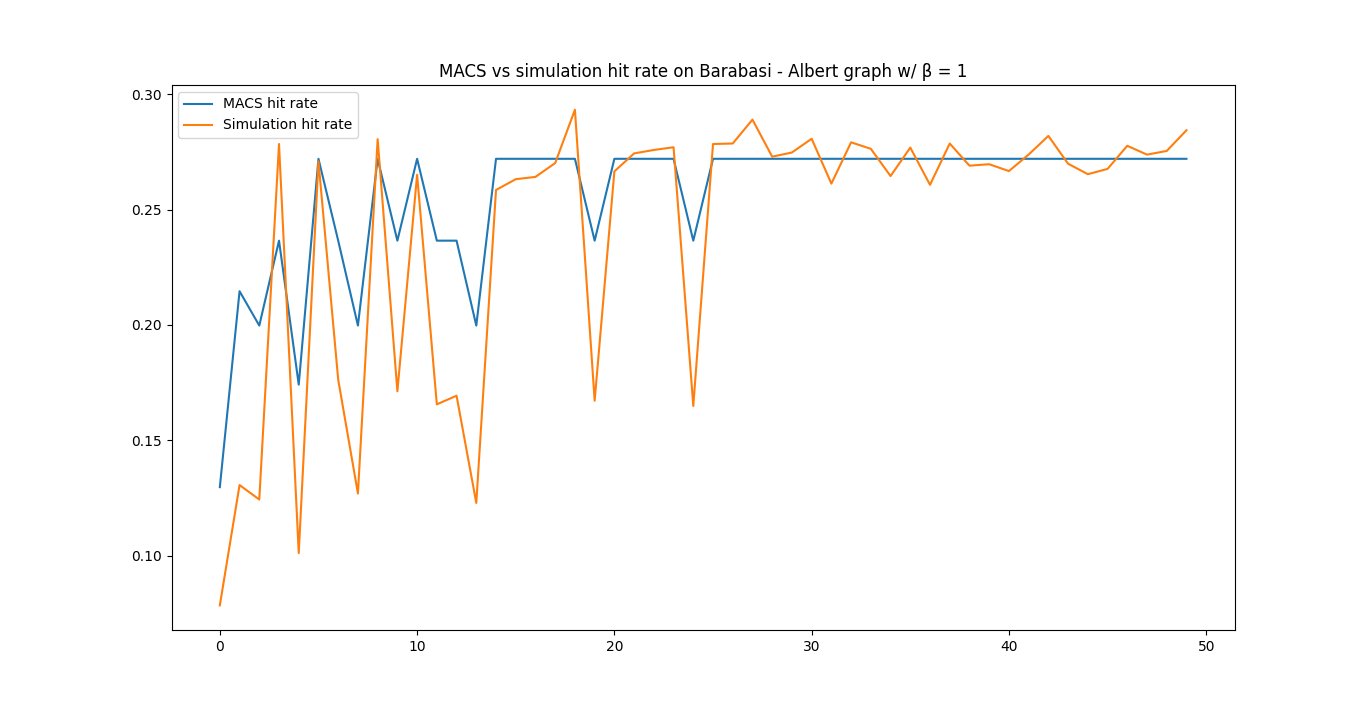
\includegraphics[scale=0.3]{ba_result.png}
    \end{figure}
\end{frame}

\begin{frame}
	\begin{center}
		\huge Thank you!
	\end{center}
\end{frame}

\end{document}